\documentclass[11pt]{article}

% Official ACL layout, with author names visible for the course submission.
\usepackage[final]{acl}
\usepackage{times}
\usepackage{latexsym}
\usepackage[T1]{fontenc}
\usepackage[utf8]{inputenc}
\usepackage{microtype}
\usepackage{inconsolata}
\usepackage{amsmath,amssymb}
\usepackage{graphicx}
\usepackage{booktabs}

% Match CodeGraph's heading hierarchy: centered sections, left-aligned
% subsections, and compact spacing before the body text.
\makeatletter
\renewcommand\section{\@startsection{section}{1}{\z@}
  {-2.0ex plus -0.5ex minus -.2ex}{0.6ex}
  {\large\bfseries\centering}}
\renewcommand\subsection{\@startsection{subsection}{2}{\z@}
  {-1.8ex plus -0.5ex minus -.2ex}{0.6ex}
  {\normalsize\bfseries\raggedright}}
\makeatother
% Keep citations and references black while preserving clickable links.
\hypersetup{hidelinks}
% Keep at least two paragraph lines together at column/page boundaries.
\clubpenalty=10000
\widowpenalty=10000
\displaywidowpenalty=10000

% Course limit: 5 pages of main content, excluding references.
% Keep the ACL margins, fonts, and body line spacing unchanged.
\title{How Invariant is Code Generation to Graph Serialization?\\
  Measuring and Localizing the Fragility}

\author{
  \normalfont
  \begin{tabular}{@{}c@{\quad}c@{\quad}c@{\quad}c@{}}
    \textbf{Ram Kedem} & \textbf{Yehonatan Barel} & \textbf{Ido Azoulay} & \textbf{Dolev Abudi} \\
    206844144 & 208646422 & 212710958 & 323096099
  \end{tabular}
}

\begin{document}
% Keep natural paragraph spacing instead of stretching gaps to fill columns.
\raggedbottom
\maketitle

\begin{abstract}
Code generation is among the strongest ways for a language model to answer a graph
question, but its invariance to how the graph is written has not been measured per
instance on executed code. We
test whether it is \emph{invariant}: we perturb one serialization axis at a time,
score every instance separately, and execute what the model writes. Across four
models and two datasets, generating code raises answer consistency under relabeling
and reordering over direct answering in 14 of 16 comparisons, yet no condition in
which the model reads the graph is invariant. The fragility is
not in transcription, which is correct in over 98\% of code records, but in the
solving program: duplicated edges are counted twice by three of the four models, and
one omitted word leads every model to build the wrong graph on one task, sometimes
still scored correct. The sensitivity is also a signal: flagging instances whose
answers disagree across permutations catches more than half of the silent errors
wherever they vary with the serialization, but almost none of a systematic error, a misread question repeated under every
serialization, which is the residual no serialization intervention here removes.
\end{abstract}

\section{Introduction}
\label{sec:introduction}
Large language models (LLMs) typically receive graphs through serialization:\ the
conversion of nodes and edges into a sequential text representation, such as a
list of edges. Renaming nodes, reordering edges, or changing the notation
preserves graph structure and query semantics while changing the token sequence
presented to the model, and prior work shows that such changes can affect
reasoning performance and lead to different answers \citep{fatemi,herbst}.

Generating and executing code offers another way to solve these problems.
Code-based approaches perform strongly on graph reasoning tasks
\citep{cai,finkelshtein}, but higher accuracy does not necessarily imply greater
invariance across serializations \citep{herbst}.

We ask: \emph{How robust are LLM-generated code solutions across different
serializations of the same graph, and what observable failures accompany a loss of
robustness?} We compare direct answering with two code modes, one that transcribes
the serialized graph into program data and one that receives the data at execution.
Per instance we score both correctness and whether the answer survives the
perturbation, since equal accuracy can hide mistakes on different questions, and we
inspect the programs for transcription, execution and logic errors.
Measurement establishes that the problem is real; localization says where it lies,
and so which remedies can apply. Our
contributions are (i) a per-instance, single-axis invariance measurement of
\emph{executed} code over four models and two datasets; (ii) a localization of the
failures in the solving program rather than in the copied graph; (iii) a graph-type omission ablation showing that a model infers an omitted graph property from
incidental nearby wording and that the resulting wrong graph can still be scored
correct; and (iv) a mitigation study on all four models in which the sensitivity
becomes an error detector, together with the error class it cannot see.

\section{Related Work}
\label{sec:related-work}
\paragraph{Graph serialization and reasoning:}
\citet{fatemi} introduce GraphQA, a benchmark of graph reasoning tasks, and
compare graph encodings and prompting strategies. Their results show that the
textual representation of a graph affects LLM performance. \citet{herbst} study invariance
more directly, decomposing serialization into node labeling, edge encoding
(including structure and order), and syntax. We build on this decomposition
and extend the comparison to LLM-generated code solutions.

\paragraph{Executing generated code:}
CodeGraph \citep{cai} generates Python for graph questions under several encodings
and so already gives evidence on encoding sensitivity in code-based reasoning; its
per-encoding accuracy comparisons motivate our complementary focus on matched
instances and on inspecting the programs. Our template is zero-shot, where CodeGraph
supplies a worked example.

\citet{finkelshtein} compare prompting, tool use and code generation and find code
generation most effective; their Graph-as-Code mode computes iteratively over a
preloaded table, and our injected-data condition adapts the idea to one program per
distinct prompt, run on data injected at execution, rather than reproducing that
protocol.

\section{Methodology}
\label{sec:methodology}

\subsection{Instances and Data}
An instance is a graph $G$, a question $q$ and a reference answer $y$; every
variant preserves both graph and query semantics. When labels change we rename the
query consistently and map node-valued answers back before scoring. The reference is
a fixed default serialization, not a canonical labeling shared by isomorphic graphs.

\paragraph{GraphQA:}
We generate undirected, unweighted graphs of 5--20 nodes from the seven families
of \citet{fatemi} (Erd\H{o}s--R\'enyi, Barab\'asi--Albert, scale-free, stochastic
block, star, path, complete). Tasks cover edge existence, node degree, node and edge
counts, neighbour and non-neighbour listing and cycle detection; questions are
sampled per graph and answers computed with NetworkX. This is a GraphQA-style
sample, not the original paper's evaluation instances.

\paragraph{Erd\H{o}s:}
Selected test tasks from \citet{guo} add harder problems: shortest paths, triangle
counting, connected components, diameter, density and bridges. The loader keeps the
original task wording and queries, recovers graph data from the prompts and checks
it against the dataset's edge field. Path predictions are additionally validated for
validity and optimal cost.
% Sources: src/gsi/data/{graphqa,erdos}.py and configs/{graphqa,erdos}.yaml.
% Frozen: GraphQA 100 graphs x 7 tasks = 700 instances (5-20 nodes, seed 0);
% Erdos 12 tasks x 100 = 1200 instances (4-34 nodes, seed 0, HF PKU-ML/Erdos test
% split, prompts <= 6000 chars). instances.jsonl is tracked in the repository.

\subsection{Serialization Perturbations}
The reference uses an edge list: GraphQA's natural-language ``adjacency''
encoding and Erd\H{o}s's native graph wording. Following \citet{herbst}, we
vary four factors: \textbf{relabeling}
permutes node identifiers; \textbf{order} changes the presentation sequence;
\textbf{structure} switches between edge lists and adjacency lists or presents
undirected edges in both directions; and \textbf{syntax} changes surface
notation, including plain text, JSON, and NetworkX code. Each variant changes
one factor only, so a difference in answers can be attributed to that factor.

Variants are built from structured graph data with fixed seeds; the generator
asserts that each changes only its designated factor and drops no-ops. Relabeling
uses a sorted identity reference and sorts again after renaming, so it holds the
ordering rule fixed rather than individual positions, and can therefore still move
edges. An instance has up to 13 forms (12 on Erd\H{o}s): the reference, the sorted
identity and three random relabelings, up to three orderings, up to two structures and up
to three syntaxes. M3 runs on all of them, but only relabeling and order change what
it receives.
% Source: src/gsi/serial/variant.py, render.py, and experiment/config.py.
% Retained forms: GraphQA 8,925 over 700 instances (12.75 per instance: 700
% canonical, 2,799 relabel, 1,926 order, 1,400 structure, 2,100 syntax); Erdos
% 14,246 over 1,200 (11.87 per instance: 1,200 / 4,799 / 3,524 / 2,323 / 2,400).
% Relabel uses 3 seeds, order 3 orderings, both after no-op removal.

\subsection{Interaction Modes}
We use three single-turn, zero-shot modes; none includes a solved example. The
modes form a ladder in which each step removes one task from the model: M1 reads
the graph, holds it, and computes; M2 delegates the computation to a program;
M3 additionally removes the copying of the graph. Figure~\ref{fig:pipeline}
shows what each mode receives and what is scored.

\begin{figure*}[t]
  \centering
  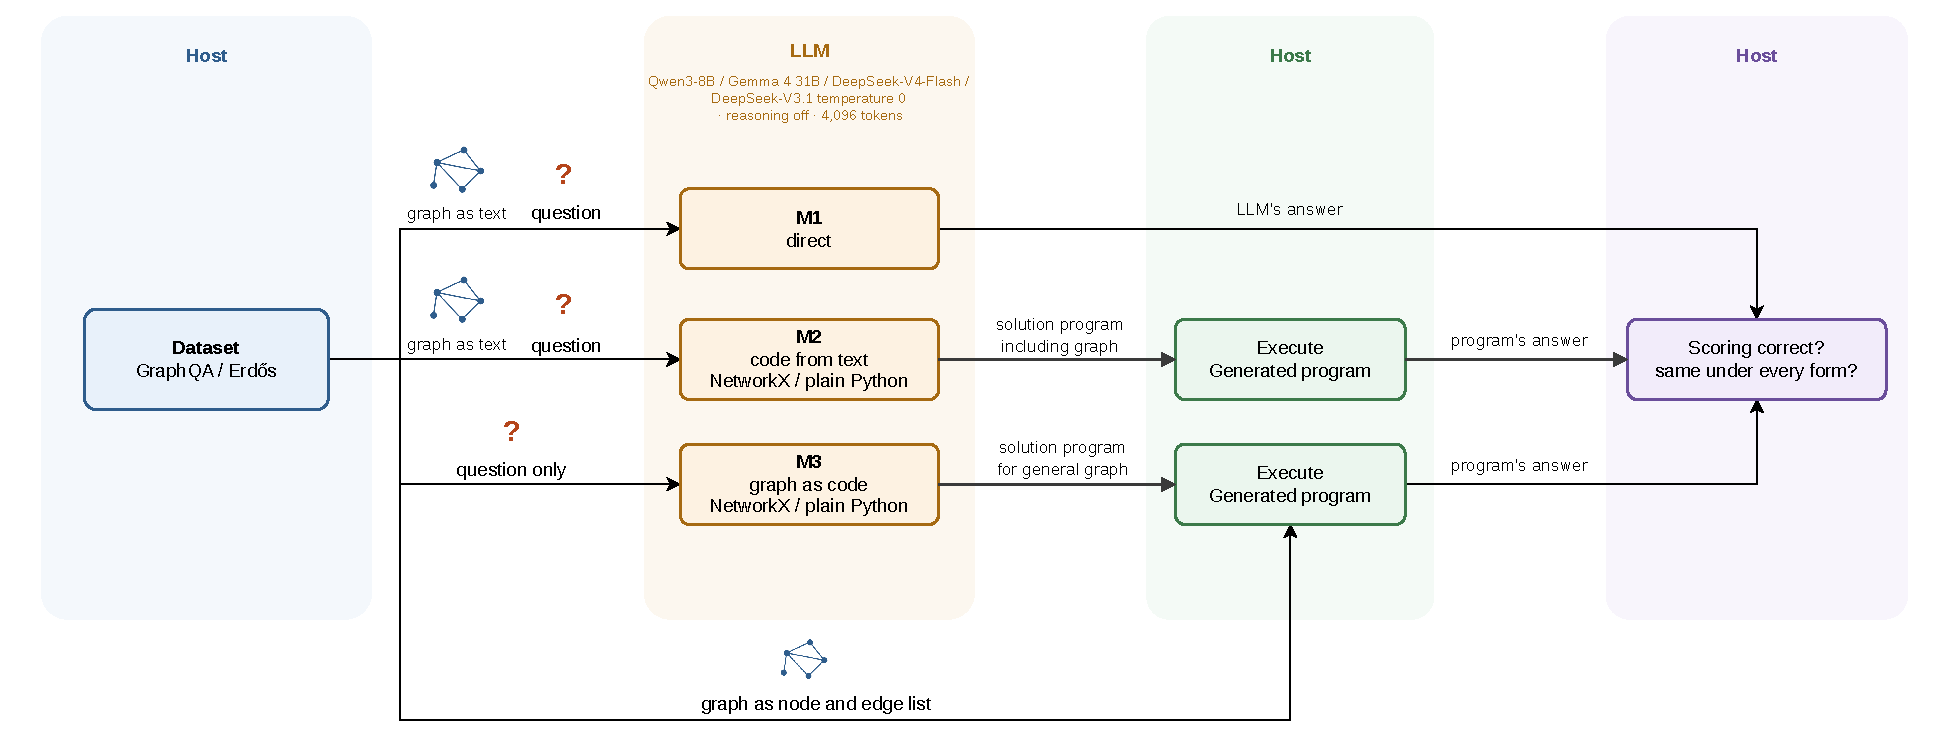
\includegraphics[width=\textwidth]{figures/pipeline_final}
  \caption{One instance through the three interaction modes and the shared scorer.}
  \label{fig:pipeline}
\end{figure*}

\paragraph{Direct answering (M1):}
Graph text and a question, with the final answer in a boxed expression. Nothing is
executed.

\paragraph{Code from text (M2):}
The same graph text as M1, and a Python template to fill: the model declares
\texttt{nodes} and \texttt{edges} first, then assigns \texttt{ans}. We execute the
code between the markers and score the value of \texttt{ans}, not printed output.
The declared lists make transcription inspectable in either library arm.

\paragraph{Graph-as-Code (M3):}
The task and question only, with instructions to use existing \texttt{nodes} and
\texttt{edges} variables whose values it never sees. The harness supplies those
lists in the variant's labels and order at execution, so M3 removes copying while
retaining construction and computation.

\paragraph{Comparing M2 and M3:}
M3 also removes the model's ability to inspect the particular graph, so an M2--M3
difference is diagnostic, not a causal estimate of transcription cost;
transcription itself is measured inside M2, from the declared lists.

Both code modes are crossed with a library arm: NetworkX permitted, or the standard
library only, which forces the algorithm to be written out. With M1 this gives five
conditions. The arms are never pooled, because they offer different tools and
different opportunities to recover intermediate graph objects.

\subsection{Failure Analysis}
We separate execution failures (including timeouts), unparseable answers and
programs that assign a literal answer without computing. Remaining wrong answers are
labelled \emph{transcription} when the declared graph differs from the input,
\emph{construction} when a recovered NetworkX graph differs from that declaration,
and otherwise \emph{logic}; programs with too little recoverable structure stay
\emph{unverifiable}. Correct answers are checked for graph mismatches separately,
since a corrupted graph can leave the queried property unchanged.

These labels are diagnostic, not a causal trace: declarations are recovered after
execution, the NetworkX object is chosen by edge overlap, edge comparisons ignore
weights and multiplicity, and in plain Python a construction error falls into
\emph{logic} because no graph object exists, so we read them per library arm.
% Source: src/gsi/score/classify.py and exec/{sandbox,runner}.py.
% The 64% / 60% of Section 5.2 are record counts (192/300, 519/872), with cache reuse.

\section{Experimental Setup}
\label{sec:setup}

\subsection{Models}
We evaluate four instruction-tuned models spanning nearly two orders of magnitude in
parameter count and three developers: Qwen3-8B (Alibaba, 8B), Gemma 4 31B (Google, 31B), and the
mixture-of-experts DeepSeek-V4-Flash (284B, 13B active) and DeepSeek-V3.1 (671B,
37B active).
% Sizes from the official Hugging Face model cards (checked 2026-09-24): Qwen3-8B
% 8.2B; Gemma 4 31B dense, 30.7B; DeepSeek-V4-Flash 284B, 13B activated; DeepSeek-V3.1
% 671B, 37B activated. configs/models.yaml lists safetensors totals (31.3B, 290.9B, 684.5B),
% which include weights the cards do not count.
% Routing/dates: Qwen3-8B via nscale (2026-09-17), DeepSeek-V3.1 via Novita
% (2026-09-18), Gemma 4 31B via Novita and DeepSeek-V4-Flash via DeepInfra
% (2026-09-19). Model ids and concurrency are pinned in configs/models.yaml.

\paragraph{Inference and execution:}
All models are served through one gateway under identical settings: temperature
zero, a 4{,}096-token limit and, where the provider exposes the switch, reasoning
disabled. Prompts are held fixed across variants except for the designated
graph/query change. Responses are cached by model and prompt text; programs run in
separate processes with a wall-clock timeout. Identical M3 prompts reuse one
generated program across many injected graphs: those are distinct evaluations but
not independent generations, though relabeling and order still affect the program's
behaviour at execution.

\paragraph{Scale:}
Every instance is evaluated in all five conditions under every retained form:
44{,}625 evaluations per model on GraphQA and 71{,}230 on Erd\H{o}s. Caching and
repeated M3 prompts leave 56--57\% of them as distinct requests.
% Distinct prompts per model: 24,942 of 44,625 (GraphQA), 40,682 of 71,230 (Erdos);
% M3 prompts carry no graph text: 1,772 distinct Erdos M3 prompts back 28,492 M3
% evaluations. accuracy.csv and invariance.csv report n_calls next to n.
% Qwen3-8B receives the "/no_think" suffix on the wire (nscale ignores the chat
% template switch); Gemma 4 31B and DeepSeek-V4-Flash disable thinking through the
% chat template; DeepSeek-V3.1 sets no switch.
% Programs run in isolated subprocesses with a 20 s wall clock and a 1 GB address
% space limit, not in Docker.

\subsection{Baselines and Metrics}
M1 is the direct-answer baseline, while M3 provides a comparison without graph
transcription. We report answer accuracy separately from program-compliance
diagnostics: a literal answer can be correct while labeled as lacking
computation. Node-valued outputs are remapped to the original labels, and
unordered answers are normalized before comparison. A floating-point prediction
$\hat{y}$ is correct when $|\hat{y}-y|\leq\max(0.01,0.01|y|)$; consistency
instead compares values rounded to four decimal places.

For instance $i$ and axis $a$, let $V_{i,a}$ hold the reference and its retained
variants and $k_{i,v}$ a normalized answer key. Then $I_{i,a}=1$ iff every answer in
$V_{i,a}$ parses and $|\{k_{i,v}\}|=1$; groups need a reference and at least one
other distinct variant. We report its mean as $I$, and the fraction correct on every
form as $R$. Consistency is not correctness: a stable wrong answer scores $I=1$, and
two equally valid shortest paths lower $I$ without lowering $R$, so the two are
always read together. Comparisons across axes must account for the differing number
of forms per instance.

Paired intervals for code-versus-direct comparisons resample graph clusters jointly
across conditions, weighting tasks and axes equally; the resulting 95\% percentile
intervals describe graph-sampling uncertainty conditional on the collected responses.
Variability under repeated identical prompts is measured separately, and invariance
is reported beside it rather than corrected by it: temperature zero is not treated as
a determinism guarantee.
% Sources: src/gsi/score/compare.py, analysis/tables.py, scripts/audit_results.py.
% Bootstrap: 5,000 paired resamples, seed 20260918, clustered by GraphQA graph id
% (100) and Erdos source path (1,179). Repeated-prompt coverage: 100 stratified (95 for the Erdos identity reference)
% instances x 4 identical asks per arm, all four models (ANALYSIS.md section 8.0);
% an unparsable repeat counts as disagreement, as in I_{i,a}. Do not subtract the
% repeated-prompt disagreement rate as if it isolated a causal effect.
% Denominators: accuracy.csv and invariance.csv report n (scored records) next to
% n_calls (distinct prompt hashes in the cell). n_calls sums per-instance counts and
% is therefore not a globally unique request count.
% Invariance-table n_calls sums per-instance counts; it is not globally unique.

\section{Results and Discussion}
\label{sec:results}

\subsection{Accuracy and Invariance}
Table~\ref{tab:main} reports $I$ and $R$ averaged over the two permutation axes.
Over the 16 code-versus-direct comparisons (four models, two datasets, two library
arms), code raises $I$ in 14 and $R$ in 15. The exceptions are on GraphQA: Gemma,
whose direct answers are already the most consistent ($97\to96$ and $95$; the
NetworkX drop, $-1.9$ points $[-3.2,-0.6]$, is significant), and
DeepSeek-V4-Flash's plain-Python $R$ ($76\to75$, within noise). The gains are largest
where direct answering is weakest: Qwen3-8B on Erd\H{o}s moves from $I=50$ to
$I=86$, and its canonical accuracy from 71\% to 95\%.

\begin{table}[t]
\centering\footnotesize
\setlength{\tabcolsep}{4pt}
\begin{tabular}{@{}lcccccc@{}}
\toprule
& \multicolumn{2}{c}{Direct} & \multicolumn{2}{c}{Native} & \multicolumn{2}{c}{NetworkX} \\
\cmidrule(lr){2-3}\cmidrule(lr){4-5}\cmidrule(lr){6-7}
Model & $I$ & $R$ & $I$ & $R$ & $I$ & $R$ \\
\midrule
\multicolumn{7}{@{}l}{\emph{GraphQA}} \\
Qwen3-8B      & 76 & 70 & 94 & 94 & 88 & 85 \\
Gemma 4 31B   & 97 & 87 & 96 & 95 & 95 & 95 \\
DeepSeek-V4-F & 90 & 76 & 93 & 75 & 92 & 79 \\
DeepSeek-V3.1 & 89 & 74 & 97 & 85 & 97 & 84 \\
\midrule
\multicolumn{7}{@{}l}{\emph{Erd\H{o}s}} \\
Qwen3-8B      & 50 & 51 & 86 & 89 & 62 & 65 \\
Gemma 4 31B   & 92 & 96 & 95 & 100 & 96 & 100 \\
DeepSeek-V4-F & 76 & 80 & 92 & 96 & 95 & 99 \\
DeepSeek-V3.1 & 84 & 88 & 94 & 98 & 92 & 97 \\
\bottomrule
\end{tabular}
\caption{Consistency $I$ and all-forms correctness $R$ (\%), averaged over
relabeling and edge order.}
\label{tab:main}
\end{table}

No condition in which the model reads the graph is invariant: the best cell is 97
(M3, which receives no graph text, reaches 100 in four of eight GraphQA arms). The
two metrics must be read
together in both directions. DeepSeek-V3.1 on GraphQA has $I=97$ but $R=85$: it
answers a different question than the benchmark intends on one task, identically
under every serialization. Its Erd\H{o}s shortest-path cell is the converse,
$I=47$ with $R=99$, because different shortest paths are equally correct.

Re-asking an identical prompt four times on about 100 stratified instances bounds how
much of the flipping is the perturbation. Every Qwen3-8B cell exceeds its own floor;
in its Erd\H{o}s plain-Python arm the floor is 0--1\% against flip rates of 8--14\%,
so essentially all of that instability is the perturbation. For the other three
models the excess is $+4$ to $+10$ points where its interval excludes zero, mostly on
relabeling, and within noise elsewhere at $n=100$: underpowered rather than null.

Presentation interacts with the condition. On GraphQA, Qwen3-8B's plain-Python
consistency is 93--96 on the permutation axes but 60 on structure, and its NetworkX
consistency falls to 61 on syntax, both below direct answering (68, 73); on
structure and syntax code trails direct answering in 5 of 32 comparisons. Gemma
stays at 94 or above on every axis in both arms.

\subsection{Failure Localization}
Transcription is not the dominant failure. The graph the program \emph{declares}
matches the input in 98.1--99.9\% of ordinary code records. It is, however, not
self-validating: among records whose declaration is wrong, 64\% (GraphQA) and 60\%
(Erd\H{o}s) still produce the correct answer, so accuracy cannot certify copying.

The failures sit in the solving code. When undirected edges are listed in both
directions, plain-Python degree code counts each edge twice in three of the four
models: accuracy falls from 99 to 5 (Qwen), 100 to 19 (DeepSeek-V3.1) and 100 to 65
(DeepSeek-V4-Flash) out of 100, while Gemma is unaffected and, with NetworkX
permitted, a \texttt{Graph} merges the duplicates (97--100). Permitting NetworkX costs
Qwen 22 points on Erd\H{o}s (69\% against 91\%), 90.7\% of its wrong NetworkX records
being execution failures, and the other three models at most one.

Finally, serialization includes what is \emph{not} written. Our injected-data
control omitted the word ``undirected'' from the Erd\H{o}s prompt. Where
the preamble asserts the graph is undirected, no program built a directed graph, and
where it says nothing only one did; where it names ``directed'' only to define a
conditional that does not apply, \emph{all four models} built a directed graph on
every undirected instance they could be observed on, and every arm scored 28/100.
Stating the type gives 100/100. The error is also partly invisible: 12 of the 84 undirected
answers were still correct, and where the preamble describes both cases Gemma built
a directed graph for 69\% of recovered graphs, nearly three quarters still correct.

\subsection{Ablations and Mitigation}
Because the fault is in the program, not the transcription, we test levers at
inference time. The first uses the sensitivity itself: flag an instance when its
answers disagree across permutations (Table~\ref{tab:detect}).

\begin{table}[t]
\centering\scriptsize
\setlength{\tabcolsep}{5pt}
\begin{tabular}{@{}llccc@{}}
\toprule
Data & Model & Flag & Caught & Abst.\ (cov.) \\
\midrule
GraphQA & Qwen3-8B      & 9.1 & 88.9 & 99.7 (90.9) \\
GraphQA & Gemma 4 31B   & 5.1 & 75.0 & 99.4 (94.9) \\
GraphQA & DeepSeek-V4-F & 9.1 & 26.3 & 82.4 (90.9) \\
GraphQA & DeepSeek-V3.1 & 3.4 & 1.1 & 86.8 (96.6) \\
Erd\H{o}s & Qwen3-8B      & 17.1 & 72.7 & 98.5 (82.9) \\
Erd\H{o}s & DeepSeek-V4-F & 9.5 & 53.8 & 99.4 (90.5) \\
Erd\H{o}s & DeepSeek-V3.1 & 8.1 & 1 of 1 & 100 (91.9) \\
Erd\H{o}s & Gemma 4 31B   & 5.0 & --- & 100 (95.0) \\
\bottomrule
\end{tabular}
\caption{Permutation disagreement as an error detector, plain-Python arm (\%).
Caught: wrong answers that returned one (a crash needs no detector).
Abst.: accuracy when answering only if all permutations agree (share answered).}
\label{tab:detect}
\end{table}

Where errors vary with the serialization it catches most of them: 73--94\% of
silent errors for Qwen and Gemma on GraphQA (both arms) and Qwen's Erd\H{o}s plain
Python at 5--17\% flag rates, where abstaining answers 83--95\% of instances at
97.3--99.8\% accuracy, and 54--56\% on Erd\H{o}s for DeepSeek-V4-Flash's plain
Python and Qwen's crash-heavy NetworkX arm. For Qwen's GraphQA plain Python one extra
relabeled call is enough: 15 of 18 errors at a 4.4\% flag rate.

The two cells where it fails are the result. Both DeepSeek models misread
\texttt{disconnected\_nodes} identically under every serialization, and it holds
59--99\% of their GraphQA errors, none caught; Gemma makes the same misreading on
only 16 graphs and 12 are caught. \emph{The blind spot is a
property of the error, not of the model.} Detection finds unstable errors, not
wrong beliefs.

Voting over the permuted answers moves code-arm accuracy by $-2.4$ to $+6.4$ points,
and voting over the permuted programs, each run on one fixed graph, by $-2.3$ to
$+5.3$ (on 300 instances per dataset): both help where errors are unstable and
amplify a majority misreading where they are not. An exact canonical labeling
renders every relabeling and reordering of every instance to one prompt; on a
fixed-stride subset covering every task (400 GraphQA and 150 Erd\H{o}s instances)
it is significantly more accurate than random labels in 8 of 24 cells and less in
one, on the ambiguous task. One solver per task, with no graph in the prompt, is free
on Erd\H{o}s for the three stronger models once told the graph type, but a single
program decides a whole task: one misread task costs each of them 3--11 points in a
GraphQA arm, and nonexistent NetworkX routines cost Qwen 4--7. A fixed adapter
reconciles the prompt's two answer conventions, dropping a solver's own top-level
call and returning an assigned but unreturned \texttt{ans}; it changes 17 Qwen
programs and no others (Qwen's GraphQA plain-Python solver: 72\% without it). A
one-sentence hint to count duplicate edges once, run later on two models against
the original run on another machine (so provider drift is not excluded), coincides
with duplicated-edge degree of 100 for DeepSeek-V3.1 (from 34 and 19) but 87 for
Qwen, whose canonical degree falls from 99 to 86 and consistency on three unrelated
axes by 6--13 points.

% Mitigation sources: ANALYSIS.md section 8 (E0-E3, E5, E6 on all four models; E4 not run; 8.5 gives the
% pre-registered criteria). Subsets take every k-th instance of instances.jsonl:
% canonical labeling 400 GraphQA (k=1: the first 58 graphs, all 7 tasks) and 150
% Erdos (k=8, 12-13 per task); program voting 300 per dataset (k=2: 86 graphs; k=4:
% 25 per task). The rendering check covers every variant of every instance. The duplicate-edge hint is on
% origin/mitigation-dedup (MITIGATION.md): Qwen3-8B and DeepSeek-V3.1 only, its
% baseline run earlier on another machine, so provider drift cannot be ruled out.
\section{Conclusion and Limitations}
\label{sec:conclusion}
Executed code is more robust than direct answering to relabeling and edge order for
most models, though not on every axis, and it is not invariant; the fragility does not enter
where expected: graphs are transcribed
almost perfectly, and the failures sit in the solving code. What remains is partly usable,
since permutation disagreement detects unstable errors at several calls per instance and
abstaining on it is nearly always right where they occur, and partly beyond these
levers: a model that misreads the question repeats that mistake under every
serialization.

We are limited to four models on one gateway, small graphs (5--20 and 4--34 nodes)
and zero-shot prompts where NetworkX is permitted, not required; every experiment
but the repeat baseline uses one generation per prompt, the deduplication hint covers two models, our pre-registered detection and per-task-solver
targets are not met, and the canonical-labeling one only for two models. Where a
question names no node, one shared M3 program can decide a task.

% Start references separately so the main-content page budget is easy to review.
\clearpage
% acl.sty selects acl_natbib; declaring the style again causes a BibTeX error.
\bibliography{references}

\end{document}
